\section{Attack classifiers}
\label{appendix:tcn}

{\small
\textbf{Beauty and Burst.}
The Beauty and the Burst classifier (BB) \cite{schuster2017beautyburst} is a CNN
(convolutional neural network) consisting of three convolution layers, a max
pooling layer, and two dense layers. We use a dropout of 0.5, 0.7, and 0.5
between the hidden layers of the network. We train the classifier with an Adam
optimizer, a categorical cross-entropy function, a learning rate of 0.01, with a
batch size of 64, and for 1000~epochs.
%\am{Show a figure?}
}

\begin{figure}[t]
    \centering
    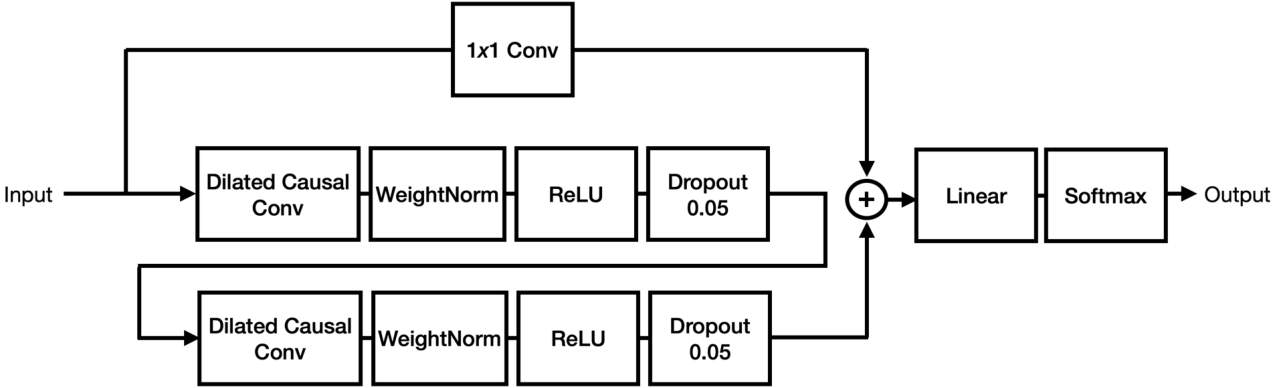
\includegraphics[width=\columnwidth]{TCN_arch.pdf}
    \caption{TCN classifier}
    \vspace{-0.4cm}
    \label{fig:tcn}
\end{figure}

{\small
\textbf{Temporal Convolution Network.}
%Recent work has proposed CNN-based classifiers for performing network
%side-channel attacks on video streams.
%While CNNs are generally effective in sequence modeling, there are two problems
%that limit their efficiency in the context of network side-channel attacks.
%First, the convolutional layers applied to a sequence are not inherently causal;
%therefore, they look into future samples of a sequence to decide the output for
%the current sample. Secondly, the effective history of past samples used by CNNs
%is bounded by the number of samples the kernel can cover, meaning the CNNs also
%lack a deep effective history size of past samples in the sequence.
%
While CNNs are generally effective in sequence modelling, they look at future
samples in a sequence and a very limited history of past samples to decide the
output of the current sample. Consequently, they require a large number of traces
and long traces for effective training and prediction.

%While CNNs are generally effective in sequence modeling, there are two problems
%that limit their efficiency in the context of network side-channel attacks.
%First, the convolutional layers need to look into future samples of a sequence
%to decide the output for the current sample, implying that they require long
%traces for effective training. Secondly, they use a limited history of past
%samples as part of training.
Temporal Convolutional Networks (TCNs) \cite{bai2018tcn} overcome these problems
of CNNs by utilizing a one-dimensional fully-convolutional network equipped with
causal dilated convolutions, which allows them to examine deep into the past to
produce an output for the sequence at any given moment.

\Cref{fig:tcn} shows the architecture of our TCN classifier, which follows the
architecture proposed by Bai et al. \cite{bai2018tcn}. It
consists of two dilated causal convolutional layers, followed by weight
normalization and dropout layers with a dropout probability of 0.05. We train
the classifier for 1000 epochs.
%\am{Show a figure?}
}

%\paragraph{Attack setup.}

\if 0
Convolutional neural networks have been shown to be effective in sequence
modelling for decades [1]. However, there are two problems with using a
convolutional neural network as a sequence modeller. First, convolutional layers
applied to a sequence are not inherently causal, meaning that they look into
future samples of a sequence to decide the output for the current sample.
Secondly, in contrast to recurrent neural networks(RNNs) [2], convolutional
neural networks lack a deep effective history size of past samples in the
sequence (i.e. their effective history is bounded to the number of samples that
kernel can cover from the past). To address these problems, Bai et al. [3]
proposed a new architecture called Temporal Convolutional Network (TCN). The TCN
utilizes a one-dimensional fully-convolutional network [4] equipped with causal
dilated convolutions [5], allowing it to examine deep into the past to produce
an output for the sequence at any given moment.  To further stabilize deep and
large TCNs, they added a generic residual block from input to output. The
architecture is shown in the following figure (it will be re-plotted for the
paper).
\fi